\documentclass[a4paper,parskip,11pt, DIV12]{scrreprt}

\usepackage[ngerman]{babel} % FÌr Deutsch [english] zu [ngerman] Àndern. 
\usepackage[utf8]{inputenc}
\usepackage[T1]{fontenc}
\usepackage{blindtext}
\usepackage{graphicx}
\usepackage{subfigure}
\renewcommand{\familydefault}{\sfdefault}
\usepackage{helvet}
\usepackage{fancyhdr}
\usepackage{amsmath}
\usepackage{mdwlist} %Benötigt fÌr AbstÀnde in AufzÀhlungen zu löschen
\usepackage{here}
\usepackage{calc}
\usepackage{hhline}
\usepackage{marginnote}
\usepackage{chngcntr}
\usepackage{tabularx}
\usepackage{titlesec} % TextÃŒberschriften anpassen

% \titleformat{Überschriftenklasse}[Absatzformatierung]{Textformatierung} {Nummerierung}{Abstand zwischen Nummerierung und Überschriftentext}{Code vor der Überschrift}[Code nach der Überschrift]

% \titlespacing{Überschriftenklasse}{Linker Einzug}{Platz oberhalb}{Platz unterhalb}[rechter Einzug]

\titleformat{\chapter}{\LARGE\bfseries}{\thechapter\quad}{0pt}{}
\titleformat{\section}{\Large\bfseries}{\thesection\quad}{0pt}{}
\titleformat{\subsection}{\large\bfseries}{\thesubsection\quad}{0pt}{}
\titleformat{\subsubsection}{\normalsize\bfseries}{\thesubsubsection\quad}{0pt}{}

\titlespacing{\chapter}{0pt}{-2em}{6pt}
\titlespacing{\section}{0pt}{6pt}{-0.2em}
\titlespacing{\subsection}{0pt}{5pt}{-0.4em}
\titlespacing{\subsubsection}{0pt}{-0.3em}{-1em}

%\usepackage[singlespacing]{setspace}
%\usepackage[onehalfspacing]{setspace}

\usepackage[
			%includemp,				%marginalien in Textkörper einbeziehen
			%includeall,
			%showframe,				%zeigt rahmen zum debuggen		
			marginparwidth=25mm, 	%breite der marginalien
			marginparsep=5mm,		%abstand marginalien - text
			reversemarginpar,		%marginalien links statt rechts
			%left=50mm,				%abstand von Seitenraendern
%			top=25mm,				%
%			bottom=50mm,
			]{geometry}		

%Bibliographie- Einstellungen
\usepackage[babel,german=quotes]{csquotes}
\usepackage[
   backend=bibtex8, 
   natbib=true,
    style=numeric,
    sorting=none
]{biblatex}
\bibliography{Quelle}
%Fertig Bibliographie- Einstellungen

\usepackage{hyperref}

\begin{document}
\selectlanguage{ngerman}
\begin{titlepage}
\begin{figure}[h]
\hfill
\subfigure{
\includegraphics[scale=0.04]{uzh}}
\end{figure}
\vspace{1 cm}
\textbf{\begin{huge}Praktikumsbericht Physik III
\end{huge}}\\
\noindent\rule{\textwidth}{1.1 pt} \\

\begin{Large}\textbf{Stern-Gerlach}
\end{Large}\\ 
\normalsize 
\par
\begingroup
\leftskip 0 cm
\rightskip\leftskip
\textbf{Modul:}\\ PHY131 \\ \\
\textbf{Assistent:}\\ Ruth Bründler\\ \\
\textbf{Studenten:}\\ Manuel Sommerhalder, Stefan Hochrein, Ruben Beynon\\ \\
\textbf{Datum des Versuchs:}\\ 22.01.2017 \\ \\
\par
\endgroup
\clearpage



\end{titlepage}


%Start Layout
\pagestyle{fancy}
\fancyhead{} 
\fancyhead[R]{\small \leftmark}
\fancyhead[C]{\textbf{Stern-Gerlach} } 
\fancyhead[L]{
\includegraphics[height=2\baselineskip]{uzh}}

\fancyfoot{}
\fancyfoot[R]{\small \thepage}
\fancyfoot[L]{}
\fancyfoot[C]{}
\renewcommand{\footrulewidth}{0.4pt} 

\addtolength{\headheight}{2\baselineskip}
\addtolength{\headheight}{0.6pt}


\renewcommand{\headrulewidth}{0.6pt}
\renewcommand{\footrulewidth}{0.4pt}
\fancypagestyle{plain}{				% plain redefinieren, damit wirklich alle seiten im gleichen stil sind (ausser titlepage)
\pagestyle{fancy}}

\renewcommand{\chaptermark}[1]{ \markboth{#1}{} } %Das aktuelle Kapitel soll nicht Gross geschriben und Nummeriertwerden

\counterwithout{figure}{chapter}
\counterwithout{table}{chapter}
%Ende Layout

\tableofcontents

\chapter{Einleitung}

Das Stern-Gerlach Experiment ist eine anschauliche Demonstration der Richtungsquantelung des magnetischen Moments aufgrund des Elektronenspins. Dazu wird ein einwertiges Metall (in unserem Fall Kalium) verdampft. Mit einer Blende entsteht ein Atomstrahl mit rechteckigem Querschnitt, der durch ein inhomogenes Magnetfeld senkrecht zu dessen Feldlinien verläuft. 
 
 Da das Kalium über abgeschlossenen inneren Schalen ein Aussenelektron hat und das magnetische Bahnmoment im Grundzustand null ist, ist das magnetische Moment des Atoms alleine auf das magnetische Spinmoment des Aussenelektrons zurückzuführen. Die Richtungsquantelung des magnetischen Moments resultiert während der Durchquerung des inhomogenen Magnetfeldes in einer symmetrischen Aufspaltung des Atomstrahls in zwei gleich grosse Teilstrahlen. Ziel des Versuchs ist es, das magnetische Moment $m_{s,z}$ anhand des Betrags der Aufspaltung, dem Gradienten des magnetischen Feldes senkrecht zur Strahlrichtung und der Geometriedaten zu bestimmen.
 
 Da zum Zeitpunkt unserer Versuchsdurchführung der Detektor defekt war, konnten wir die Messung leider nicht selbst durchführen. Daher verwendeten wir die Messdaten einer anderen Gruppe. Die Bilder stammen alle aus der Versuchsanleitung.
 
 \section{Überlegungen zum Versuch}
 
 Vor der Versuchsdurchführung waren folgende Fragen zu beantworten:
 
 \textit{1. Stern und Gerlach haben 1921 in ihrem Experiment Silber verwendet. Warum funktioniert der
Versuch auch mit Kalium?}

Sowohl Silber, als auch Kalium verfügen über ein einzelnes Aussenelektron über abgeschlossenen inneren Schalen und haben im Grundzustand kein magnetisches Bahnmoment, wodurch das magnetische Moment alleine durch das magnetische Spinmoment des Aussenelektrons zustande kommt.

\textit{2. Welche Vor- und Nachteile hat die Verwendung von Kalium gegenüber von Silber?}

Der Vorteil von Kalium gegenüber Silber liegt in der viel geringeren Temperatur, die zur Verdampfung nötig ist. Die Temperatur, die für Silber notwendig wäre, bedürfte einerseits einer aufwendigeren Beheizung und wäre andererseits entscheidend schwieriger konstant zu halten. Der Nachteil von Kalium liegt hingegen in der heftigen Reaktionsfreudigkeit. Wenn kein Hochvakuum in der Apparatur bestehen würde, würden sofort stark exotherme Oxidationen stattfinden.

\textit{3. Welche weiteren Elemente könnten theoretisch verwendet werden?}

Theoretisch sollte der Versuch mit allen Elementen der ersten und elften Gruppe des Periodensystems durchführbar sein, da diese die bei Frage 1 diskutierten Kriterien erfüllen. in der Praxis sind diese Elemente jedoch unterschiedlich gut geeignet, beispielsweise wäre von der Verwendung des radioaktiven Elements Roentgenium abzuraten.

\textit{4. Warum funktioniert dieser Versuch nicht mit einem Elektronenstrahl?}

Im Gegensatz zu den verwendeten Atomen hat das Elektron eine negative Ladung, aufgrund derer es sogleich aufgrund der Lorentz-Kraft im magnetischen Feld abgelenkt werden würde.

\textit{5. Warum funktioniert dieser Versuch nicht mit einem homogenen Magnetfeld?}

Bei Verwendung eines homogenen Magnetfeldes würde das magnetische Moment sich lediglich beim Eintritt in das Feld ausrichten und sich dann geradlinig weiterbewegen. Für eine konstante Kraft während des ganzen Aufenthalts im Feld ist ein konstanter Feldgradient vonnöten, der nur in einem inhomogenen Magnetfeld bestehen kann.

\section{Versuchsaufbau und Methodik}
	\begin{figure}[H]
\centering
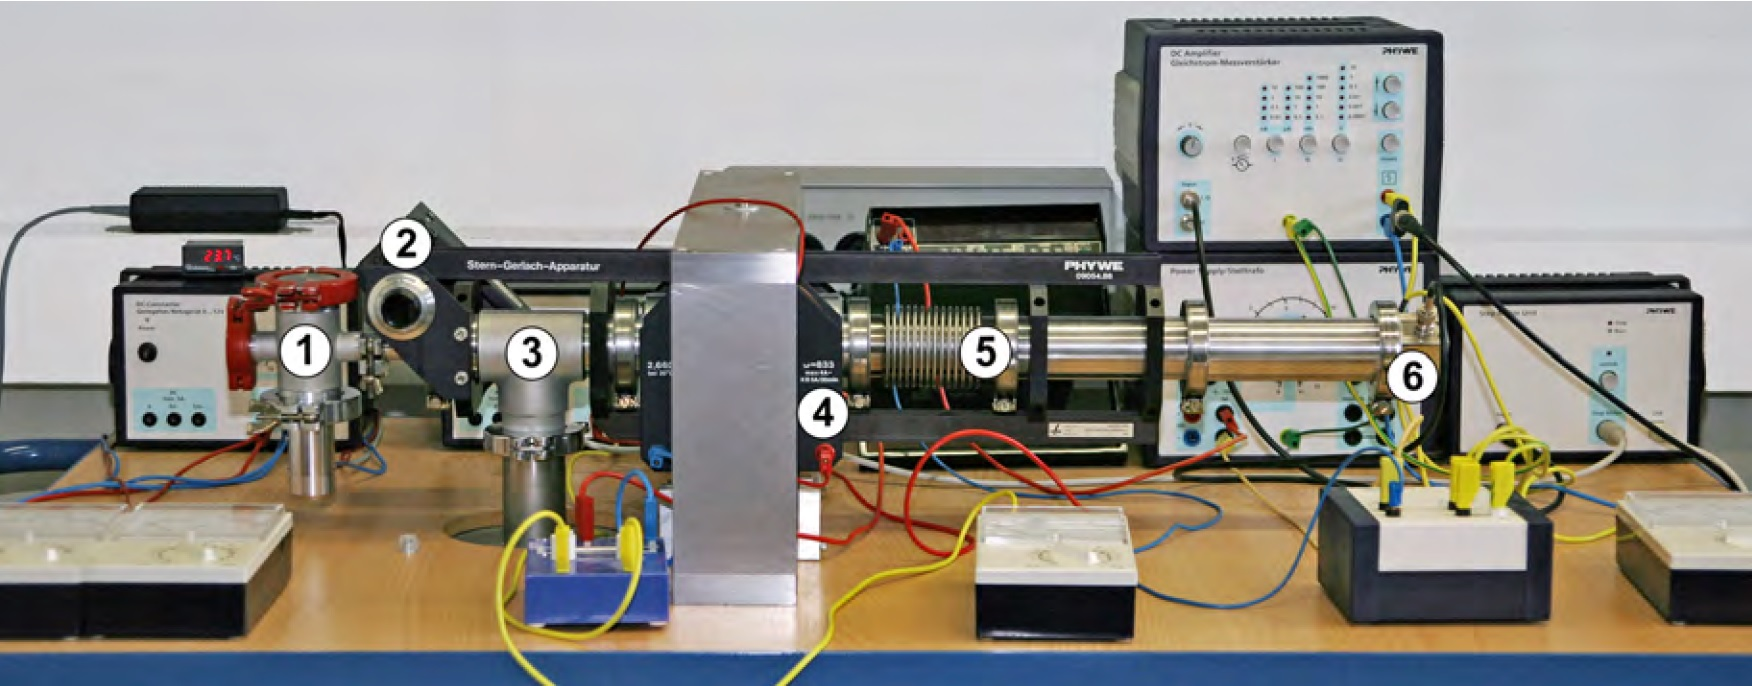
\includegraphics[keepaspectratio,width=\textwidth,height=\textheight]{Setup}
\caption[Setup]{Versuchsanordnung}
\label{Abb:Setup}
\end{figure}
Abbildung \ref{Abb:Setup} gibt einen Überblick über die wichtigsten Elemente des Versuchsaufbaus. Um eine Oxidierung des Kaliums zu verhindern, wird die Apparatur durch den Pumpenanschluss (3) evakuiert (unter 5$\cdot$10$^{-6}$ mbar). Der Ofen (1) wird auf ca 460 K aufgeheizt. Da die Temperatur trotz Regelung Schwankungen unterliegt, wird diese bei jeder Messung an der Messanzeige abgelesen und notiert. Der Strom auf den magnetischen Analysator (4) wird bei jeder Messung aufwärts variiert, um den Einfluss verschiedener Feldstärken beobachten zu können. Das Atomstrahlrohr (5) ist an der lamellierten Stelle nach dem Analysator biegbar, wodurch der Langmuir-Taylor-Detektor (6) per Schritttmotor (2) bewegt werden kann. Dadurch kann der Detektor per Computerprogramm gesteuert innerhalb eines Intervalls bei gleichmässiger Geschwindigkeit alle Positionen $u$ durchlaufen und die entsprechende Teilchenstromdichte $J(u)$ messen. 

	Mit Hilfe des vorgegebenen Matlab-Tools wird dann mit dem Levenberg-Marquardt-Algorithmus ein Fit durch die Messdaten gelegt, dessen Form einer Überlagerung der in der Versuchsanleitung hergeleiteten theoretischen Verteilung und der des Nullfeldes entspricht. Diese Kurve verfügt über zwei lokalen Maxima, deren Abstand $q$ für die Berechnung des magnetischen Moments $m_{s,z}$ verwendet wird.

\clearpage

\chapter{Messdaten}

\section{Datentabelle}
In Tabelle \ref{tabelle1} sind die wichtigsten Resultate der Messungen zusammengefasst, und zwar der Strom $I$ durch die Magnetspulen, die Magnetfeldstärke $B$, die der jeweiligen Stromstärke $I$ entspricht (bestimmt anhand der Magnetfeld-Eichkurve in der Versuchsanleitung), die abgelesene Temperatur $T$ des Ofens und der Abstand $q$ zwischen den lokalen Maxima des Fits. Wir beschränken uns an dieser Stelle auf diese zusammengefasste Darstellung der Daten, da die Originalmessdaten pro Messung mehrere tausend Messpunkte umfassen. \\

\begin{table}[H]
\centering
\renewcommand{\arraystretch}{1.2} % Abstandzwischen Zeilen
\setlength{\tabcolsep}{3mm} % Abstandzwischen Spalten
\begin{tabular}{|c|c|c|c|} 
$I$ [mA] & $B$ [T] & $T$ [K]  & $q$ [mm]\\ \hline
402   $\pm$ 5      & 0.320   $\pm$ 0.010   & 457.3  $\pm$ 0.1   & 2.2452 $\pm$ 0.0015 \\
600    $\pm$ 5      & 0.485   $\pm$ 0.010   & 459.5  $\pm$ 0.1   &3.5437  $\pm$ 0.0025\\
700    $\pm$ 5      & 0.560   $\pm$ 0.010  & 459.7   $\pm$ 0.1   &4.2096  $\pm$ 0.0029\\
800    $\pm$ 5     & 0.635    $\pm$ 0.010 & 459.7    $\pm$ 0.1   & 4.7810 $\pm$  0.0032 \\
900    $\pm$ 5     & 0.695    $\pm$ 0.010 & 459.9    $\pm$ 0.1    &5.3034  $\pm$  0.0032 \\
1000    $\pm$ 5    & 0.750     $\pm$ 0.010 & 460.7       $\pm$ 0.1 &5.7311  $\pm$ 0.0041
\end{tabular}
\caption[Daten]{Zusammenfassung der Daten}\label{tabelle1}
\end{table} Für die Berechnung des magnetischen Moments des Elektrons haben wir ausserdem die folgenden im Datenblatt der Versuchsanleitung gegebenen Konstanten verwendet:

Länge der Pole:
$L$ = (70.0 $\pm$ 0.5) mm

Radius des konvexen Pols:
$a$ = (2.5 $\pm$ 0.2) mm

Distanz Magnetfeldeintritt-Detektor:
$l$ = (0.455 $\pm$ 0.001) m

Proportionalitätsfaktor zwischen dem Magnetfeld und seiner Änderung in z-Richtung:\\
$\epsilon$ = 0.9530 $\pm$ 0.0026

\section{Fehlerabschätzung}
Der Fehler auf den Strom $m_I$ ist anhand der Anzeigegenauigkeit des Messgerätes abgeschätzt und fliesst nur indirekt in die Fehlerrechnung. Der Fehler auf die magnetische Induktion $m_B$ setzt sich zusammen aus dem Fehler auf dem Strom $m_I$ und der Ungenauigkeit des Ablesens aus der Kurve. Der Fehler auf der Temperatur wurde als höher abgeschätzt als die Ungenauigkeit des Messgerätes, da die Temperatur trotz aller Bemühungen zur Konstanthaltung während einer Messung dennoch leicht variieren konnte. Der Fehler auf den Abstand der lokalen Maxima $m_q$ ergibt sich aus dem Algorithmus der Fit-Methode.

Die Fehler auf den Längen $L$, $l$ und $a$ haben wir anhand ihrer Grösse und der Schwierigkeit der Durchführung der Messung abgeschätzt. Der Fehler auf $\epsilon$ ist aus den Praktikumsunterlagen bekannt.
\clearpage

\chapter{Resultate}
In Tabelle \ref{tabelle2} sind die in Kapitel \ref{Datenanalyse} errechneten Werte und deren Fehler (aus Kapitel \ref{Fehlerrechnung}) des magnetischen Moments des Elektrons $m_{s,z}$ mit den entsprechenden magnetischen Feldstärken $B$ zusammengefasst. Dabei ist augenfällig, dass der Betrag von $m_{s,z}$ mit der Feldstärke $B$ zunimmt.\\

\begin{table}[H]
\centering
\renewcommand{\arraystretch}{1.2} % Abstandzwischen Zeilen
\setlength{\tabcolsep}{3mm} % Abstandzwischen Spalten
\begin{tabular}{|c|c|}
$B$ [T] & $m_{s,z}$ [10$^{-24}$ J$\cdot$T$^{-1}$] \\ \hline
0.320 $\pm$ 0.010 & -7.90 $\pm$ 0.68\\
0.485 $\pm$ 0.010 & -8.27 $\pm$ 0.68\\
0.560 $\pm$ 0.010 & -8.51 $\pm$ 0.70\\
0.635 $\pm$ 0.010 & -8.53 $\pm$ 0.70\\
0.695 $\pm$ 0.010 & -8.65 $\pm$ 0.70\\
0.750 $\pm$ 0.010 & -8.67 $\pm$ 0.70\\
\end{tabular}
\caption[Resultate]{Errechnete Werte für $m_{s,z}$ zu verschiedenen Feldstärken $B$}\label{tabelle2}
\end{table} Der daraus errechnete Mittelwert ist:$\quad \overline{m}_{s,z}$ = (-8.42 $\pm$ 0.69) $\cdot$ 10$^{-24}$ J$\cdot$T$^{-1}$

Wenn wir dies mit dem Literaturwert\footnote{National Institute of Standards and Technology, http://physics.nist.gov/cgi-bin/cuu/Value?muem, abgerufen am 9.2.17} $m_{s,z}$ = -9.28 $\cdot$ 10$^{-24}$ J$\cdot$T$^{-1}$ vergleichen, so sehen wir, dass dieser knapp nicht in der Fehlergrenze unseres Wertes liegt. Mögliche Fehlerquellen sehen wir in der schwankenden Temperatur des Ofens und den eventuell schlecht kalibrierten Geräten. Auch mag in der Vereinfachung in Formel \ref{BGradient} zur Bestimmung des Feldgradienten eine grobe Fehlerquelle liegen, die nicht in der Fehlerrechnung berücksichtigt wurde. Nichtsdestotrotz zeichneten sich deutlich zwei diskrete lokale Maxima ab, was die Aufspaltung aufgrund der zwei verschiedenen Spineinstellungen immerhin qualitativ nachweisen konnte.


\clearpage


\chapter{Datenanalyse}\label{Datenanalyse}

Aus Überlegungen zum geometrischen Aufbau der Versuchsanlage und der Kraft eines räumlich variierenden Magnetfeldes auf ein magnetisches Moment $\vec{ \mu }$ ergibt sich Formel (4.1), welche wir aus der Versuchsanleitung übernommen haben. Dabei sind $u_e$ die wahrscheinlichsten Aufprallpunkte der Atome und $q$ ist der Abstand der beiden Maxima, die sich aus den zwei Spineinstellungen ergeben, $L$ ist die Länge der Pole, $l$ die Distanz zwischen Magnetfeldeintritt und Detektor, $a$ der Radius des konvexen Pols, $k_B$ die Boltzmann-Konstante und $T$ die Temperatur.


\begin{equation}
u_e=\pm \frac{q}{3}=\frac{lL(1-\frac{L}{2l})m_{s,z} \frac{\partial B}{\partial z}}{6k_BT}
\end{equation}

Die Veränderung des Magnetfeld in $z$-Richtung ergibt sich aus der Geometrie der Polschuhe (Abbildung \ref{Abb:Polschuhe}). Dabei ist der Aufbau des Magneten so gewählt, dass sich ein möglichst konstanter Gradient in $z$-Richtung entlang des Atomstrahls ergibt.

\begin{figure}[H]
\centering
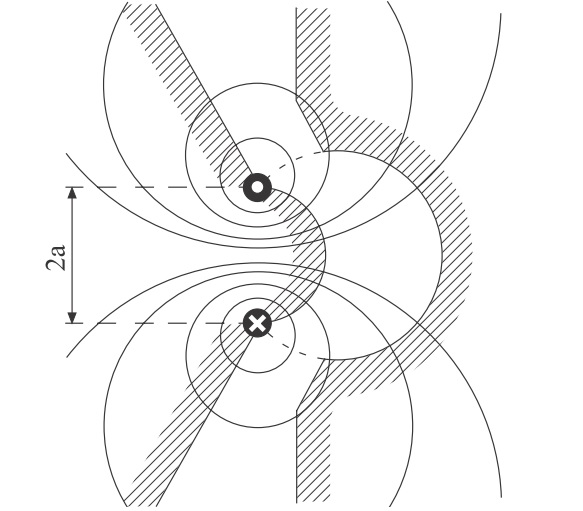
\includegraphics[scale=0.7]{Polschuhe}
\caption[Polschuhe]{Geometrie der Polschuhe}
\label{Abb:Polschuhe}
\end{figure} Aufgrund der Tatsache, dass der Gradient eines Magnetfeld schwer zu messen ist, wurde die Annahme getroffen, dass $\frac{ \partial B}{ \partial z}$ proportional zu $B$ ist für kleine Auslenkungen in $z$. Daraus ergibt sich der Proportionalitätsfaktor $\epsilon$.

\begin{equation} \label{BGradient}
\epsilon = \left|\frac{\partial B}{\partial z}\right| \frac{a}{B}
\end{equation}

Damit leiteten wir folgende Formel zur Berechnung des magnetischen Moments des Elektrons $m_{s,z}$ her:
\begin{equation} \label{Moment}
m_{s,z}=\frac{2k_BTqa}{lL(1-\frac{L}{2l})\epsilon B}
\end{equation}

Anhand von Formel \ref{Moment} wurden somit zu den jeweiligen Werten von $B$, $q$ und $T$ die das magnetische Moment des Elektrons $m_{s,z}$ berechnet und in Tabelle \ref{tabelle2} zusammengefasst.

\clearpage

\chapter{Fehlerrechnung} \label{Fehlerrechnung}
Die Fehlerfortpflanzung wurde nach dem Gauss'schen Fehlerfortpflanzungsgesetz (Formel \ref{Gauss}) durchgeführt. Dabei haben wir nur die Fehler auf $q$, $a$, $\epsilon$ und $B$ in unsere Berechnung einbezogen. Die Fehler auf der Temperatur $T$ und den Aufbaukonstanten $L$ und $l$ haben wir vernachlässigt, weil eine Verdoppelung des jeweiligen Fehlers nur eine Veränderung in der dritten Nachkommastelle des Gesamtfehlers zur Folge hatte.


\begin{equation} \label{Gauss}
m_{m_{s,z}}=\sqrt{(\frac{\partial m}{\partial q} \cdot m_q)^2+(\frac{\partial m}{\partial a} \cdot m_a)^2+(\frac{\partial m}{\partial \epsilon} \cdot m_\epsilon)^2+(\frac{\partial m}{\partial B} \cdot m_B)^2}
\end{equation}

Die folgenden vier Gleichungen (\ref{ersteableitung} bis \ref{letzteableitung}) sind die Partiellen Ableitungen der Formel \ref{Moment}, welche wir zur Berechnung des Gesamtfehlers auf $m_{s,z}$ benötigt haben.

\begin{equation} \label{ersteableitung}
\frac{\partial m}{\partial q} = \frac{2k_BTa}{lL(1-\frac{L}{2l})\epsilon B}
\end{equation}

\begin{equation}
\frac{\partial m}{\partial a} = \frac{2k_BTq}{lL(1-\frac{L}{2l})\epsilon B}
\end{equation}

\begin{equation}
\frac{\partial m}{\partial \epsilon} = \frac{-2k_BTaq}{lL(1-\frac{L}{2l})\epsilon^2 B}
\end{equation}

\begin{equation} \label{letzteableitung}
\frac{\partial m}{\partial B} = \frac{-2k_BTaq}{lL(1-\frac{L}{2l})\epsilon B^2}
\end{equation}


\clearpage
 

%\renewcommand{\bibname}{Quellenverzeichnis}
%\printbibliography

\end{document}
